\documentclass[11pt]{charter}

% El títulos de la memoria, se usa en la carátula y se puede usar el cualquier lugar del documento con el comando \ttitle
\titulo{ID Mobile - Sistema de identificación personal para teléfono móvil, mediante Bluetooth} 

% Nombre del posgrado, se usa en la carátula y se puede usar el cualquier lugar del documento con el comando \degreename
%\posgrado{Carrera de Especialización en Sistemas Embebidos} 
\posgrado{Carrera de Especialización en Internet de las Cosas} 
%\posgrado{Carrera de Especialización en Intelegencia Artificial}
%\posgrado{Maestría en Sistemas Embebidos} 
%\posgrado{Maestría en Internet de las cosas}

% Tu nombre, se puede usar el cualquier lugar del documento con el comando \authorname
\autor{Rosito Pedro} 

% El nombre del director y co-director, se puede usar el cualquier lugar del documento con el comando \supname y \cosupname y \pertesupname y \pertecosupname
\director{Nelson Fortunatti}
\pertenenciaDirector{ITBA} 
% FIXME:NO IMPLEMENTADO EL CODIRECTOR ni su pertenencia
\codirector{} % si queda vacio no se deberíá incluir 
\pertenenciaCoDirector{}

% Nombre del cliente, quien va a aprobar los resultados del proyecto, se puede usar con el comando \clientename y \empclientename
\cliente{Sergio Starkloff}
\empresaCliente{SURiX SRL}

% Nombre y pertenencia de los jurados, se pueden usar el cualquier lugar del documento con el comando \jurunoname, \jurdosname y \jurtresname y \perteunoname, \pertedosname y \pertetresname.
\juradoUno{Nombre y Apellido (1)}
\pertenenciaJurUno{pertenencia (1)} 
\juradoDos{Nombre y Apellido (2)}
\pertenenciaJurDos{pertenencia (2)}
\juradoTres{Nombre y Apellido (3)}
\pertenenciaJurTres{pertenencia (3)}
 
\fechaINICIO{25 de agosto de 2020}		%Fecha de inicio de la cursada de GdP \fechaInicioName
\fechaFINALPlanificacion{13 de octubre de 2020} 	%Fecha de final de cursada de GdP
\fechaFINALTrabajo{22 de julio de 2021}		%Fecha de defensa pública del trabajo final


\begin{document}

\maketitle
\thispagestyle{empty}
\pagebreak


\thispagestyle{empty}
{\setlength{\parskip}{0pt}
\tableofcontents{}
}
\pagebreak


\section{Registros de cambios}
\label{sec:registro}


\begin{table}[ht]
\label{tab:registro}
\centering
\begin{tabularx}{\linewidth}{@{}|c|X|c|@{}}
\hline
\rowcolor[HTML]{C0C0C0} 
Revisión & \multicolumn{1}{c|}{\cellcolor[HTML]{C0C0C0}Detalles de los cambios realizados} & Fecha      \\ \hline
1.0      & Creación del documento                                          & 25/08/2020 \\ \hline
1.1      & Se completó la descripción del proyecto & 2/09/2020 \\ \hline
1.2      & Se completaron parcialmente los puntos del 1 al 6 & 3/09/2020 \\ \hline
1.3		& Se terminó con los puntos del 1 al 6 y se completó la identificación y análisis de los interesados & 6/09/2020 \\ \hline
\end{tabularx}
\end{table}

\pagebreak



\section{Acta de constitución del proyecto}
\label{sec:acta}

\begin{flushright}
Buenos Aires, \fechaInicioName
\end{flushright}

\vspace{2cm}

Por medio de la presente se acuerda con el Ing. \authorname\hspace{1px} que su Trabajo Final de la \degreename\hspace{1px} se titulará ``\ttitle'', consistirá esencialmente en un sistema de identificación mobile utilizando tecnología bluetooth, y tendrá un presupuesto preliminar estimado de 600 hs de trabajo y \textcolor{red}{\$XXX}, con fecha de inicio \fechaInicioName\hspace{1px} y fecha de presentación pública \fechaFinalName.

Se adjunta a esta acta la planificación inicial.

\vfill

% Esta parte se construye sola con la información que hayan cargado en el preámbulo del documento y no debe modificarla
\begin{table}[ht]
\centering
\begin{tabular}{ccc}
\begin{tabular}[c]{@{}c@{}}Ariel Lutenberg \\ Director posgrado FIUBA\end{tabular} & \hspace{2cm} & \begin{tabular}[c]{@{}c@{}}\clientename \\ \empclientename \end{tabular} \vspace{2.5cm} \\ 
\multicolumn{3}{c}{\begin{tabular}[c]{@{}c@{}} \supname \\ Director del Trabajo Final\end{tabular}} \vspace{2.5cm} \\
%\begin{tabular}[c]{@{}c@{}}\jurunoname \\ Jurado del Trabajo Final\end{tabular}     &  & \begin{tabular}[c]{@{}c@{}}\jurdosname\\ Jurado del Trabajo Final\end{tabular}  \vspace{2.5cm}  \\
%\multicolumn{3}{c}{\begin{tabular}[c]{@{}c@{}} \jurtresname\\ Jurado del Trabajo Final\end{tabular}} \vspace{.5cm}                                                                     
\end{tabular}
\end{table}




\section{Descripción técnica-conceptual del proyecto a realizar}
\label{sec:descripcion}

Surix es una empresa que se dedica al diseño y venta de porteros IP para el uso domiciliario, hospitalario y empresarial. 
Entre sus productos se destacan diferentes tipos de porteros, algunos de ellos presentan la posibilidad de manejarse mediante un celular con una aplicación llamada VoIPBell. Ésta aplicación tiene la limitación de poder manejar un sólo portero a la vez. \newline
Teniendo en cuenta que estamos frente a un contexto de cambio tecnológico en el mundo donde cada vez más servicios se pueden incluir en un celular y realizar de manera automatizada, se presenta un panoráma ideal para plantear avances en materia de comododiad funcional en aspectos de la vida diaria. \newline
Éste proyecto de ID Mobile viene a aportar la posibilidad de contar con una aplicación en la que los usuarios puedan crearse una cuenta mediante la cuál puedan tener acceso a todas las puertas en las que tengan instalado un portero bluetooth, puede ser tanto de su casa como de su trabajo. Teniendo la posibilidad de programarlas, para que se abran a cierta hora de forma periódica, para dar acceso de única vez, para hacer control de rondas, etc. La aplicación propuesta se comunicará con un servidor el cuál tendrá acceso a una base de datos en la cuál estarán guardadas las cuentas de los diferentes usuarios, ya sean administradores o usuarios llanos. A su vez la base de datos tendrá conocimiento, previa carga por parte del usuario, de todas las puertas bluetooth instaladas, de manera de poder asociarlas a los usuarios correspondientes. En la Figura 1 se muestra un diagrama de bloques en el que se puede observar el funcionamiento del sistema. 

\vspace{25px}

\begin{figure}[htpb]
\centering 
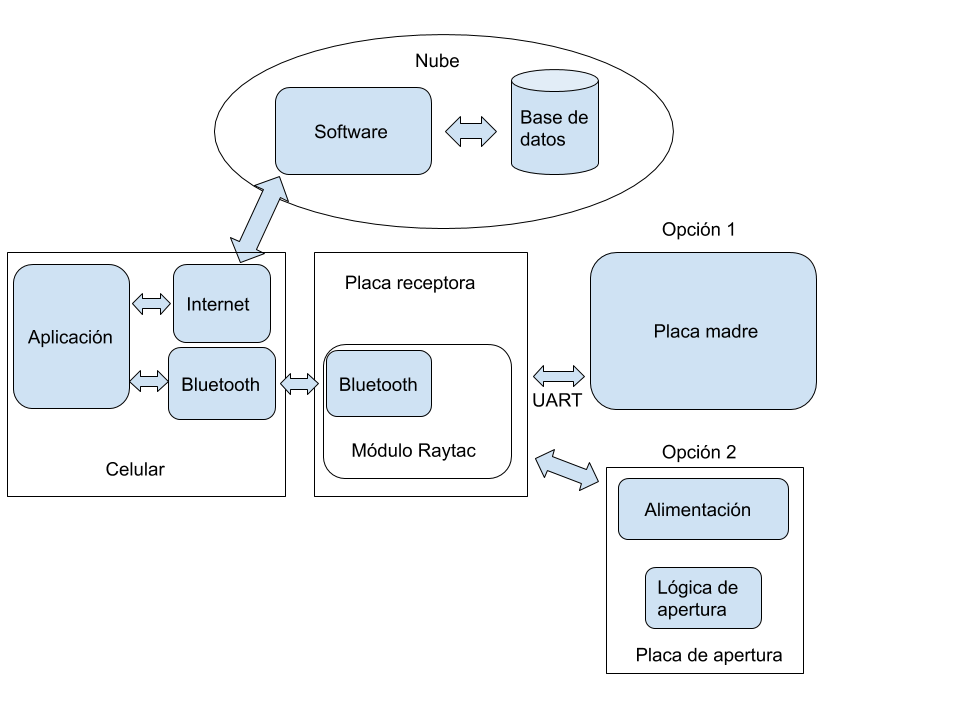
\includegraphics[width=.9\textwidth]{./Figuras/Diagramadebloques_planificacion.png}
\caption{Diagrama en bloques del sistema ID Mobile}
\label{fig:diagBloques}
\end{figure}

\vspace{25px}

Observamos en la figura que existen dos opciones, opción 1 y opción 2, esto se debe a que el sistema se vendera como parte de un sistema mayor comandando por una placa madre (portero) que conocerá los permisos de cada usuario y en base a eso decidirá que acciones se deben llevar a cabo una vez recibida la señal por parte de la placa receptora (opción 1) o por otra parte el sistema se venderá de forma standalone, es decir que existirá la placa receptora junto con la placa de apertura asociadas a una puerta y la aplicación será la que decida a partir de lo comunicado por el software en la nube si la puerta en cuestión puede o no abrirse (opción 2).



\section{Identificación y análisis de los interesados}
\label{sec:interesados}


\begin{table}[ht]
%\caption{Identificación de los interesados}
%\label{tab:interesados}
\begin{tabularx}{\linewidth}{@{}|l|X|X|l|@{}}
\hline
\rowcolor[HTML]{C0C0C0} 
Rol           & Nombre y Apellido & Organización 	& Puesto 	\\ \hline
Cliente       & \clientename      &\empclientename	& CTO       	\\ \hline
Responsable   & \authorname       & FIUBA        	& Alumno 	\\ \hline
Orientador    & \supname	      & \pertesupname 	& Director	Trabajo final \\ \hline
Colaborador        & Raúl Camacho      & SURiX SRL       & Desarrollador de software        	\\ \hline
\end{tabularx}
\end{table}


\begin{itemize}
\item Sergio Starkloff: No se encuentra actualmente en Argentina, pero a pesar de la diferencia horaria practicamente siempre está disponible para hacerle consultas. Está muy atento a todo lo referente al proyecto y siempre llega con nuevas propuestas e ideas. 
\item Nelson Fortunatti: Tiene mucho conocimiento de programación de microprocesadores por lo que su orientación será fundamental al momento de crear el software para la placa.
\item Raúl Camacho: Trabajaremos juntos en el diseño del hardware del proyecto, ya que es compartido con su trabajo de especialización.
\end{itemize}





\section{1. Propósito del proyecto}
\label{sec:proposito}


El propósito de éste proyecto es el de crear un sistema nuevo para la empresa, aprovechando la conectividad con la que cuentan prácticamente todos los celulares hoy en dia, abriendo la posibilidad de comenzar con una rama de productos orientada al internet de las cosas.


\section{2. Alcance del proyecto}
\label{sec:alcance}


En éste proyecto se incluye:
\begin{itemize}
\item El diseño de la placa receptora, utilizando un módulo previamente adquirido por la empresa, a través de un esquemático en Kicad.
\item El diseño de la placa de apertura, a través de un esquemático en Kicad.
\item La programación de un software en la placa receptora para la comunicación vía bluetooth con un celular.
\item La creación de un software en aws (o algún servicio en la nube a determinar).
\item La creación de una base de datos en aws (o algún servicio en la nube a determinar).
\item La creación de una aplicación que pueda funcionar tanto en iOS como en Android.
\end{itemize}
En éste proyecto no se incluye:
\begin{itemize}
\item El diseño del pcb de las placas ni la implementación física de las mismas.
\item Ninguna etapa del diseño ni implementación de la placa madre.
\end{itemize}


\section{3. Supuestos del proyecto}
\label{sec:supuestos}

Para el desarrollo del presente proyecto se supone que:

\begin{itemize}
\item Las placas estarán implementadas en tiempo y forma para poder realizar las pruebas necesarias.
\item La programación de la aplicación que pueda funcionar en Android e iOS no será demasiado compleja para el tiempo estimado de realización de la tarea.
\item La complejidad de la programación del software para la placa receptora no será demasiado elevada para el tiempo estimado de realización de la tarea.
\item Será posible implementar todas las funciones requeridas para la aplicación.
\end{itemize}


\section{4. Requerimientos}
\label{sec:requerimientos}


\begin{enumerate}
\item Requerimientos asociados con la placa receptora.
	\begin{enumerate}
	\item Podrá comunicarse mediante bluetooth con un celular.
	\item Será capaz de recibir alimentación y comunicarse mediante UART con una placa madre.
	\item Será capaz de recibir alimentación y comunicarse mediante 5 pines con una placa de apertura.
	\item Dispondrá de un jumper para cambiar de comportamiento para los dos casos anteriores.
	\item Podrá enviar una orden de apertura a la placa de apertura mediante un tren de pulsos.
	\item La lógica de apertura no puede ser simulada de forma externa para evitar el vandalismo o robo.
	\end{enumerate}
\item Requerimientos asociados con la placa de apertura.
	\begin{enumerate}
	\item Será capaz de alimentar y comunicarse mediante 5 pines con la placa receptora.
	\item Podrá interpretar el tren de pulsos enviado por la placa receptora mediante un circuito contador o alguna lógica sencilla.
	\item Contará con un relé que se utilizará para abrir la puerta.
	\item Contará con una bocina para avisar de la apertura de la puerta.
	\item Podrá ser alimentada con 12V de alterna o continua.
	\end{enumerate}
\item Requerimientos asociados con la aplicación (mínimo producto viable)
	\begin{enumerate}
	\item Deberá ser capaz de comunicarse por bluetooth con la placa receptora y mediante internet con el software en la nube.
	\item Deberá presentar una interfaz de usuario mediante la cuál gestionar el uso de las puertas disponibles.
	\item Deberá constituir un consumo muy bajo para la batería del celular.
	\item Se debe comunicar periódicamente con el software en la nube para revalidar permisos.
	\item La comunicación entre la aplicación y la placa receptora debe ser segura.
	\end{enumerate}
\item Requerimientos asociados con el sistema.
	\begin{enumerate}
	\item Debe funcionar en la nube (aws o alguna otra a determinar).
	\item Debe permitir a los usuarios crear una cuenta y asociarla a sus puertas.
	\item Debe permitir a los usuarios administrar sus puertas, cargándolas o eliminándolas del sistema, dando permisos a otros usuarios ya sea de forma periódica, de única vez o en franjas horarias determinadas.
	\item Debe permitir la configuración de la cuenta creada (cambiar foto, nombre, contraseña, etc.)
	\item Debe poder generar reportes de movimiento, tanto de usuarios como de cerraduras.
	\end{enumerate}
\end{enumerate}


\section{Historias de usuarios (\textit{Product backlog})}
\label{sec:backlog}

\begin{consigna}{red}
Descripción: En esta sección se deben incluir las historias de usuarios y su ponderación (\textit{history points}). Recordar que las historias de usuarios son descripciones cortas y simples de una característica contada desde la perspectiva de la persona que desea la nueva capacidad, generalmente un usuario o cliente del sistema. La ponderación es un número entero que representa el tamaño de la historia comparada con otras historias de similar tipo.
\end{consigna}

\section{5. Entregables principales del proyecto}
\label{sec:entregables}

\begin{itemize}
\item Esquemático de las placas receptora y de apertura.
\item Aplicación funcional para Android e iOS.
\item Software para la placa receptora que cumpla con los requerimientos especificados.
\item Software y base de datos en la nube.
\item Repositorio con el código fuente utilizado.
\item Documentación referente al código creado.

\end{itemize}


\section{6. Desglose del trabajo en tareas}
\label{sec:wbs}


\begin{enumerate}
\item Planificación del proyecto (30 hs)
	\begin{enumerate}
	\item Reuniones con el cliente para acordar los diferentes puntos. (5 hs)
	\item Estudio de los requerimientos planteados por el cliente (15 hs)
	\item Creación de la documentación. (10 hs)
	\end{enumerate}
\item Investigación previa (100 hs)
	\begin{enumerate}
	\item Estudio del módulo MDBT42Q de Raytac. (20 hs)
	\item Estudio y preparación del SDK de Nordic para el desarrollo del software en placa. (20 hs)
	\item Estudio sobre programación en la nube. (20 hs)
	\item Estudio sobre el protocolo de comunicación bluetooth. (20 hs)
	\item Estudio sobre la programación de aplicaciones híbridas. (20hs)
	\end{enumerate}
\item Selección de recursos a utilizar (55 hs)
	\begin{enumerate}
	\item Selección de la nube de alguna compañia. (10 hs)
	\item Selección de componentes para el diseño de las placas. (15 hs)
	\item Selección de los lenguajes de programación a utilizar. (15 hs)
	\item Selección de los entornos de trabajo para la realización del software. (15 hs)
	\end{enumerate}
\item Desarrollo del hardware (60 hs)
	\begin{enumerate}
	\item Realización de la lógica para la apertura de la puerta (20 hs)
	\item Realización del esquemático de la placa receptora. (20 hs)
	\item Realización del esquemático de la placa de apertura. (20 hs)
	\end{enumerate}
\item Desarrollo del software (275 hs)
	\begin{enumerate}
	\item Desarrollo del software en la nube (65 hs)
		\begin{enumerate}
		\item Desarrollo de la interfaz principal de usuario. (10 hs)
		\item Desarrollo de la interfaz y funcionalidad para la creación de cuenta. (15 hs)
		\item Desarrollo de la interfaz y funcionalidad para la configuración de cuenta. (25 hs)
		\item Desarrollo de la comunicación con la base de datos. (15 hs)
		\end{enumerate}
	\item Desarrollo de la aplicación (140 hs)
		\begin{enumerate}
		\item Desarrollo de la interfaz principal de usuario. (20 hs)
		\item Comunicación con bluetooth para Android e iOS. (30 hs)
		\item Desarrollo de la interfaz y funcionalidad para la creación de cuenta. (20 hs)
		\item Desarrollo de la interfaz y funcionalidad para la configuración de cuenta. (30 hs)
		\item Integración y depuración del código para su funcionamiento tanto en Android como en iOS. (40 hs)
		\end{enumerate}
	\item Implementación de la base de datos en la nube. (30 hs)
	\item Desarrollo del software en la placa receptora. (40 hs)
	\end{enumerate}
\item Pruebas de integración (105 hs)
	\begin{enumerate}
	\item Implementación de la comunicación entre el software en la nube y la aplicación. (35 hs)
	\item Implementación de la comunicación vía bluetooth entre el software en la placa y la aplicación. (35 hs)
	\item Implementación y pruebas del sistema completo. (35 hs)
	\end{enumerate}
	
\end{enumerate}

Cantidad total de horas: (625 hs)


\section{7. Diagrama de Activity On Node}
\label{sec:AoN}

\begin{consigna}{red}
Armar el AoN a partir del WBS definido en la etapa anterior. 

%La figura \ref{fig:AoN} fue elaborada con el paquete latex tikz y pueden consultar la siguiente referencia \textit{online}:

%\url{https://www.overleaf.com/learn/latex/LaTeX_Graphics_using_TikZ:_A_Tutorial_for_Beginners_(Part_3)\%E2\%80\%94Creating_Flowcharts}

\end{consigna}

\begin{figure}[htpb]
\centering 
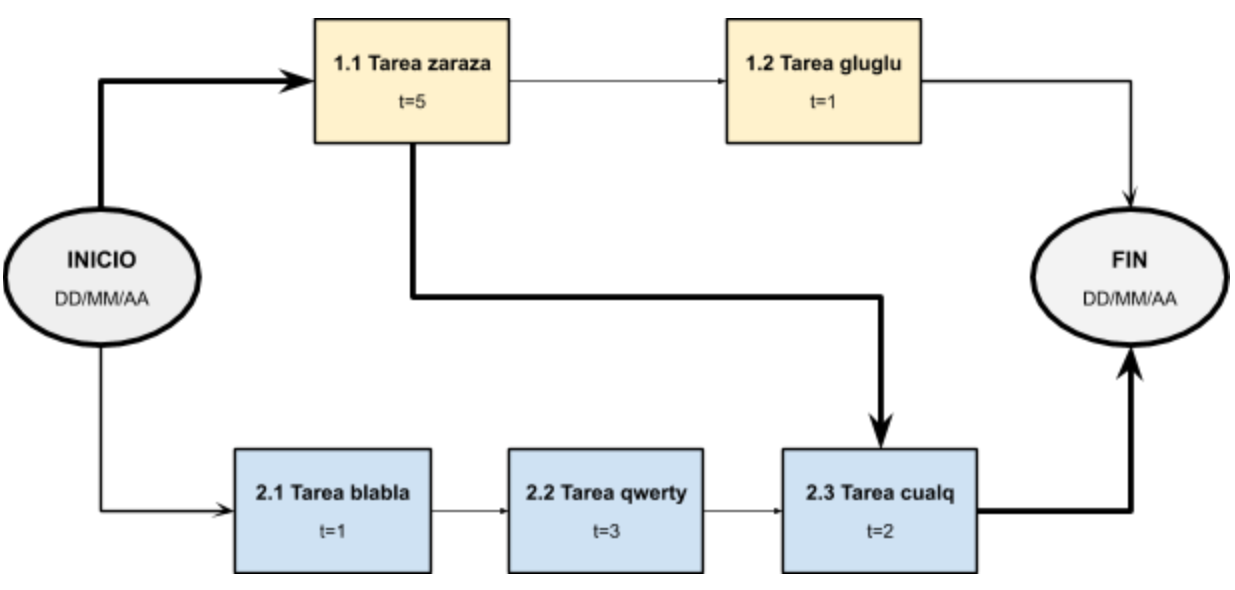
\includegraphics[width=.8\textwidth]{./Figuras/AoN.png}
\caption{Diagrama en \textit{Activity on Node}}
\label{fig:AoN}
\end{figure}

Indicar claramente en qué unidades están expresados los tiempos.
De ser necesario indicar los caminos semicríticos y analizar sus tiempos mediante un cuadro.
Es recomendable usar colores y un cuadro indicativo describiendo qué representa cada color, como se muestra en el siguiente ejemplo:



\section{8. Diagrama de Gantt}
\label{sec:gantt}

\begin{consigna}{red}
Utilizar el software Gantter for Google Drive o alguno similar para dibujar el diagrama de Gantt.

Existen muchos programas y recursos \textit{online} para hacer diagramas de gantt, entre las cuales destacamos:

\begin{itemize}
\item Planner
\item GanttProject
\item Trello + \textit{plugins}. En el siguiente link hay un tutorial oficial: \\ \url{https://blog.trello.com/es/diagrama-de-gantt-de-un-proyecto}
\item Creately, herramienta online colaborativa. \\\url{https://creately.com/diagram/example/ieb3p3ml/LaTeX}
\item Se puede hacer en latex con el paquete \textit{pgfgantt}\\ \url{http://ctan.dcc.uchile.cl/graphics/pgf/contrib/pgfgantt/pgfgantt.pdf}
\end{itemize}

Pegar acá una captura de pantalla del diagrama de Gantt, cuidando que la letra sea suficientemente grande como para ser legible. 
Si el diagrama queda demasiado ancho, se puede pegar primero la ``tabla'' del Gantt y luego pegar la parte del diagrama de barras del diagrama de Gantt.

Configurar el software para que en la parte de la tabla muestre los códigos del EDT (WBS).\\
Configurar el software para que al lado de cada barra muestre el nombre de cada tarea.\\
Revisar que la fecha de finalización coincida con lo indicado en el Acta Constitutiva.

En la figura \ref{fig:gantt}, se muestra un ejemplo de diagrama de gantt realizado con el paquete de \textit{pgfgantt}. En la plantilla pueden ver el código que lo genera y usarlo de base para construir el propio.

\begin{figure}[htbp]
\begin{center}
\begin{ganttchart}{1}{12}
  \gantttitle{2020}{12} \\
  \gantttitlelist{1,...,12}{1} \\
  \ganttgroup{Group 1}{1}{7} \\
  \ganttbar{Task 1}{1}{2} \\
  \ganttlinkedbar{Task 2}{3}{7} \ganttnewline
  \ganttmilestone{Milestone o hito}{7} \ganttnewline
  \ganttbar{Final Task}{8}{12}
  \ganttlink{elem2}{elem3}
  \ganttlink{elem3}{elem4}
\end{ganttchart}
\end{center}
\caption{Diagrama de gantt de ejemplo}
\label{fig:gantt}
\end{figure}

\end{consigna}

\section{9. Matriz de uso de recursos de materiales}
\label{sec:recursos}


\begin{table}
\label{tab:recursos}
\centering
\begin{tabularx}{\linewidth}{@{}|c|X|X|X|X|c|@{}}
\hline
\cellcolor[HTML]{C0C0C0} & \cellcolor[HTML]{C0C0C0} & \multicolumn{4}{c|}{\cellcolor[HTML]{C0C0C0}Recursos requeridos (horas)} \\ \cline{3-6} 
\multirow{-2}{*}{\cellcolor[HTML]{C0C0C0}\begin{tabular}[c]{@{}c@{}}Código\\ WBS\end{tabular}} & \multirow{-2}{*}{\cellcolor[HTML]{C0C0C0}\begin{tabular}[c]{@{}c@{}}Nombre \\ tarea\end{tabular}} & Material 1 & Material 2 & Material 3 & Material 4 \\ \hline
 &  &  &  &  &  \\ \hline
 &  &  &  &  &  \\ \hline
 &  &  &  &  &  \\ \hline
 &  &  &  &  &  \\ \hline
 &  &  &  &  &  \\ \hline
 &  &  &  &  &  \\ \hline
 &  &  &  &  &  \\ \hline
 &  &  &  &  &  \\ \hline 
 &  &  &  &  &  \\ \hline
 &  &  &  &  &  \\ \hline
 &  &  &  &  &  \\ \hline
 &  &  &  &  &  \\ \hline
 &  &  &  &  &  \\ \hline
 &  &  &  &  &  \\ \hline
 &  &  &  &  &  \\ \hline
 &  &  &  &  &  \\ \hline
 &  &  &  &  &  \\ \hline
 &  &  &  &  &  \\ \hline
 &  &  &  &  &  \\ \hline
 &  &  &  &  &  \\ \hline
 &  &  &  &  &  \\ \hline
 &  &  &  &  &  \\ \hline
 &  &  &  &  &  \\ \hline
 &  &  &  &  &  \\ \hline 
 &  &  &  &  &  \\ \hline
 &  &  &  &  &  \\ \hline
 &  &  &  &  &  \\ \hline
 &  &  &  &  &  \\ \hline

\end{tabularx}%
\end{table}


\section{10. Presupuesto detallado del proyecto}
\label{sec:presupuesto}

\begin{consigna}{red}
Si el proyecto es complejo entonces separarlo en partes:
\begin{itemize}
\item Un total global, indicando el subtotal acumulado por cada una de las áreas.
\item El desglose detallado del subtotal de cada una de las áreas.
\end{itemize}

IMPORTANTE: No olvidarse de considerar los COSTOS INDIRECTOS.

\end{consigna}

\begin{table}[htpb]
\centering
\begin{tabularx}{\linewidth}{@{}|X|c|r|r|@{}}
\hline
\rowcolor[HTML]{C0C0C0} 
\multicolumn{4}{|c|}{\cellcolor[HTML]{C0C0C0}COSTOS DIRECTOS} \\ \hline
\rowcolor[HTML]{C0C0C0} 
Descripción &
  \multicolumn{1}{c|}{\cellcolor[HTML]{C0C0C0}Cantidad} &
  \multicolumn{1}{c|}{\cellcolor[HTML]{C0C0C0}Valor unitario} &
  \multicolumn{1}{c|}{\cellcolor[HTML]{C0C0C0}Valor total} \\ \hline
 &
  \multicolumn{1}{c|}{} &
  \multicolumn{1}{c|}{} &
  \multicolumn{1}{c|}{} \\ \hline
 &
  \multicolumn{1}{c|}{} &
  \multicolumn{1}{c|}{} &
  \multicolumn{1}{c|}{} \\ \hline
\multicolumn{1}{|l|}{} &
   &
   &
   \\ \hline
\multicolumn{1}{|l|}{} &
   &
   &
   \\ \hline
\multicolumn{3}{|c|}{SUBTOTAL} &
  \multicolumn{1}{c|}{} \\ \hline
\rowcolor[HTML]{C0C0C0} 
\multicolumn{4}{|c|}{\cellcolor[HTML]{C0C0C0}COSTOS INDIRECTOS} \\ \hline
\rowcolor[HTML]{C0C0C0} 
Descripción &
  \multicolumn{1}{c|}{\cellcolor[HTML]{C0C0C0}Cantidad} &
  \multicolumn{1}{c|}{\cellcolor[HTML]{C0C0C0}Valor unitario} &
  \multicolumn{1}{c|}{\cellcolor[HTML]{C0C0C0}Valor total} \\ \hline
\multicolumn{1}{|l|}{} &
   &
   &
   \\ \hline
\multicolumn{1}{|l|}{} &
   &
   &
   \\ \hline
\multicolumn{1}{|l|}{} &
   &
   &
   \\ \hline
\multicolumn{3}{|c|}{SUBTOTAL} &
  \multicolumn{1}{c|}{} \\ \hline
\rowcolor[HTML]{C0C0C0}
\multicolumn{3}{|c|}{TOTAL} &
   \\ \hline
\end{tabularx}%
\end{table}


\section{11. Matriz de asignación de responsabilidades}
\label{sec:responsabilidades}
\begin{consigna}{red}
Establecer la matriz de asignación de responsabilidades y el manejo de la autoridad completando la siguiente tabla:

\begin{table}[htpb]
\centering
\resizebox{\textwidth}{!}{%
\begin{tabular}{|c|c|c|c|c|c|}
\hline
\rowcolor[HTML]{C0C0C0} 
\cellcolor[HTML]{C0C0C0} &
  \cellcolor[HTML]{C0C0C0} &
  \multicolumn{4}{c|}{\cellcolor[HTML]{C0C0C0}Listar todos los nombres y roles del proyecto} \\ \cline{3-6} 
\rowcolor[HTML]{C0C0C0} 
\cellcolor[HTML]{C0C0C0} &
  \cellcolor[HTML]{C0C0C0} &
  Responsable &
  Orientador &
  Equipo &
  Cliente \\ \cline{3-6} 
\rowcolor[HTML]{C0C0C0} 
\multirow{-3}{*}{\cellcolor[HTML]{C0C0C0}\begin{tabular}[c]{@{}c@{}}Código\\ WBS\end{tabular}} &
  \multirow{-3}{*}{\cellcolor[HTML]{C0C0C0}Nombre de la tarea} &
  \authorname &
  \supname &
  Nombre de alguien &
  \clientename \\ \hline
 &  &  &  &  &  \\ \hline
 &  &  &  &  &  \\ \hline
 &  &  &  &  &  \\ \hline
\end{tabular}%
}
\end{table}

{\footnotesize
Referencias:
\begin{itemize}
	\item P = Responsabilidad Primaria
	\item S = Responsabilidad Secundaria
	\item A = Aprobación
	\item I = Informado
	\item C = Consultado
\end{itemize}
} %footnotesize

Una de las columnas debe ser para el Director, ya que se supone que participará en el proyecto.
A su vez se debe cuidar que no queden muchas tareas seguidas sin ``A'' o ``I''.

Importante: es redundante poner ``I/A'' o ``I/C'', porque para aprobarlo o responder consultas primero la persona debe ser informada.

\end{consigna}

\section{12. Gestión de riesgos}
\label{sec:riesgos}

\begin{consigna}{red}
a) Identificación de los riesgos (al menos cinco) y estimación de sus consecuencias:
 
Riesgo 1: detallar el riesgo (riesgo es algo que si ocurre altera los planes previstos)
\begin{itemize}
\item Severidad (S): mientras más severo, más alto es el número (usar números del 1 al 10).\\
Justificar el motivo por el cual se asigna determinado número de severidad (S).
\item Probabilidad de ocurrencia (O): mientras más probable, más alto es el número (usar del 1 al 10).\\
Justificar el motivo por el cual se asigna determinado número de (O). 
\end{itemize}   

Riesgo 2:
\begin{itemize}
\item Severidad (S): 
\item Ocurrencia (O):
\end{itemize}

Riesgo 3:
\begin{itemize}
\item Severidad (S): 
\item Ocurrencia (O):
\end{itemize}


b) Tabla de gestión de riesgos:      (El RPN se calcula como RPN=SxO)

\begin{table}[htpb]
\centering
\begin{tabularx}{\linewidth}{@{}|X|c|c|c|c|c|c|@{}}
\hline
\rowcolor[HTML]{C0C0C0} 
Riesgo & S & O & RPN & S* & O* & RPN* \\ \hline
       &   &   &     &    &    &      \\ \hline
       &   &   &     &    &    &      \\ \hline
       &   &   &     &    &    &      \\ \hline
       &   &   &     &    &    &      \\ \hline
       &   &   &     &    &    &      \\ \hline
\end{tabularx}%
\end{table}

Criterio adoptado: 
Se tomarán medidas de mitigación en los riesgos cuyos números de RPN sean mayores a...

Nota: los valores marcados con (*) en la tabla corresponden luego de haber aplicado la mitigación.

c) Plan de mitigación de los riesgos que originalmente excedían el RPN máximo establecido:
 
Riesgo 1: plan de mitigación (si por el RPN fuera necesario elaborar un plan de mitigación).
  Nueva asignación de S y O, con su respectiva justificación:
  - Severidad (S): mientras más severo, más alto es el número (usar números del 1 al 10).
          Justificar el motivo por el cual se asigna determinado número de severidad (S).
  - Probabilidad de ocurrencia (O): mientras más probable, más alto es el número (usar del 1 al 10).
          Justificar el motivo por el cual se asigna determinado número de (O).

Riesgo 2: plan de mitigación (si por el RPN fuera necesario elaborar un plan de mitigación).
 
Riesgo 3: plan de mitigación (si por el RPN fuera necesario elaborar un plan de mitigación).

\end{consigna}


\section{13. Gestión de la calidad}
\label{sec:calidad}

\begin{consigna}{red}
Para cada uno de los requerimientos del proyecto indique:
\begin{itemize} 
\item Req \#1: copiar acá el requerimiento.

Verificación y validación:

\begin{itemize}
\item Verificación para confirmar si se cumplió con lo requerido antes de mostrar el sistema al cliente. Detallar 
\item Validación con el cliente para confirmar que está de acuerdo en que se cumplió con lo requerido. Detallar  
\end{itemize}

\end{itemize}

Tener en cuenta que en este contexto se pueden mencionar simulaciones, cálculos, revisión de hojas de datos, consulta con expertos, mediciones, etc.

\end{consigna}

\section{14. Comunicación del proyecto}
\label{sec:comunicaciones}

El plan de comunicación del proyecto es el siguiente:

\begin{table}[htpb]
\centering
\begin{tabularx}{\linewidth}{@{}|X|C{2.4cm}|C{3cm}|C{1.8cm}|C{2cm}|C{2.1cm}|@{}}
\hline
\rowcolor[HTML]{C0C0C0} 
\multicolumn{6}{|c|}{\cellcolor[HTML]{C0C0C0}PLAN DE COMUNICACIÓN DEL PROYECTO}           \\ \hline
\rowcolor[HTML]{C0C0C0} 
¿Qué comunicar? & Audiencia & Propósito & Frecuencia & Método de comunicac. & Responsable \\ \hline
                &           &           &            &                      &             \\ \hline
                &           &           &            &                      &             \\ \hline
                &           &           &            &                      &             \\ \hline
                &           &           &            &                      &             \\ \hline
                &           &           &            &                      &             \\ \hline
\end{tabularx}
\end{table}

\section{15. Gestión de compras}
\label{sec:compras}

\begin{consigna}{red}
En caso de tener que comprar elementos o contratar servicios:
a) Explique con qué criterios elegiría a un proveedor.
b) Redacte el Statement of Work correspondiente.
\end{consigna}

\section{16. Seguimiento y control}
\label{sec:seguimiento}

\begin{consigna}{red}
Para cada tarea del proyecto establecer la frecuencia y los indicadores con los se seguirá su avance y quién será el responsable de hacer dicho seguimiento y a quién debe comunicarse la situación (en concordancia con el Plan de Comunicación del proyecto).

El indicador de avance tiene que ser algo medible, mejor incluso si se puede medir en \% de avance. Por ejemplo,se pueden indicar en esta columna cosas como ``cantidad de conexiones ruteadeas'' o ``cantidad de funciones implementadas'', pero no algo genérico y ambiguo como ``\%'', porque el lector no sabe porcentaje de qué cosa.

\end{consigna}

\begin{longtable}{|m{1cm}|m{3.5cm}|m{2.2cm}|m{2cm}|m{3cm}|m{1.5cm}|}
\hline
\rowcolor[HTML]{C0C0C0} 
\multicolumn{6}{|c|}{\cellcolor[HTML]{C0C0C0}SEGUIMIENTO DE AVANCE}                                                                       \\ \hline
\rowcolor[HTML]{C0C0C0} 
Tarea del WBS 			& Indicador de avance & Frecuencia de reporte & Resp. de seguimiento & Persona a ser informada & Método de comunic. \\ \hline
\endfirsthead

\hline
\rowcolor[HTML]{C0C0C0} 
\multicolumn{6}{c}{\cellcolor[HTML]{C0C0C0}SEGUIMIENTO DE AVANCE}                                                                       \\ \hline
\rowcolor[HTML]{C0C0C0} 
Tarea del WBS 			& Indicador de avance & Frecuencia de reporte & Resp. de seguimiento & Persona a ser informada & Método de comunic. \\ \hline
\endhead

\multicolumn{6}{c}{Continúa}
\endfoot

\endlastfoot

1.1	& Fecha de inicio  & Única vez al comienzo & \authorname & \clientename, \supname & email \\ \hline
2.1	& Avance de las subtareas  & Mensual mientras dure la tarea & \authorname & \clientename, \supname & email \\ \hline

\end{longtable}

\begin{table}[!htpb]
\centering
%\begin{tabularx}{\linewidth}{@{}|X|X|X|X|X|X|@{}}
\begin{tabularx}{\linewidth}{@{}|X|C{2.5cm}|C{3cm}|C{2cm}|C{2cm}|C{2.5cm}|@{}}
\hline
\rowcolor[HTML]{C0C0C0} 
\multicolumn{6}{|c|}{\cellcolor[HTML]{C0C0C0}SEGUIMIENTO DE AVANCE}                                                                       \\ \hline
\rowcolor[HTML]{C0C0C0} 
Tarea del WBS & Indicador de avance & Frecuencia de reporte & Resp. de seguimiento & Persona a ser informada & Método de comunic. \\ \hline
 &  &  &  &  &  \\ \hline
 &  &  &  &  &  \\ \hline
 &  &  &  &  &  \\ \hline
 &  &  &  &  &  \\ \hline
 &  &  &  &  &  \\ \hline
\end{tabularx}%
%}
\end{table}

\section{17. Procesos de cierre}    
\label{sec:cierre}

\begin{consigna}{red}
Establecer las pautas de trabajo para realizar una reunión final de evaluación del proyecto, tal que contemple las siguientes actividades:

\begin{itemize}
\item Pautas de trabajo que se seguirán para analizar si se respetó el Plan de Proyecto original:
 - Indicar quién se ocupará de hacer esto y cuál será el procedimiento a aplicar. 
\item Identificación de las técnicas y procedimientos útiles e inútiles que se utilizaron, y los problemas que surgieron y cómo se solucionaron:
 - Indicar quién se ocupará de hacer esto y cuál será el procedimiento para dejar registro.
\item Indicar quién organizará el acto de agradecimiento a todos los interesados, y en especial al equipo de trabajo y colaboradores:
  - Indicar esto y quién financiará los gastos correspondientes.
\end{itemize}

\end{consigna}


\end{document}
